\section{A Series of Tubes}

\subsection{Tool for Tube Design}

We created a tool which novice designers can use to create tube-powered interfaces in arbitrary 3D models.  This tool allows users to brush over the surface of their model to either select exterior connection points of their tubes (see Figure \ref{fig:tool-process-interior}) or to author the tubes' interior paths (see Figure \ref{fig:tool-process-exterior}).  Once the user's selections are made, our tool creates an initial shortest-path routing using A* to estimate the routed distance between points.  This routing is used to create a rod; we run physics-based simulation steps on the rod to minimize its bending energy (and thereby minimize the bend radius of the tubes).  The resultant routing is subtracted from the user's mesh.  The modified mesh can then be 3D printed.

\subsubsection{Selection}

\textbf{Exterior Connection Points}

\begin{figure}[h!]
\centering
    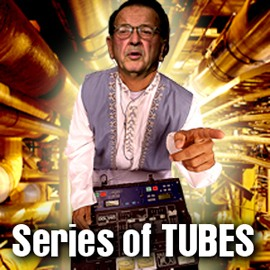
\includegraphics[width=3.4in]{figures/series-of-tubes.jpg}
\caption{This figure has several sub-figures.  a) shows a model with exterior connection points brushed.  b) shows initial routing with A*.  c) shows our physics-based, energy-minimizing rod/tube, d) shows the printed object with the tube (with something in it, copper paint presumably)}
\label{fig:tool-process-exterior}
\end{figure}

Focus on shape of points and location of points.

\textbf{Designing Interior Paths}

\begin{figure}[h!]
\centering
    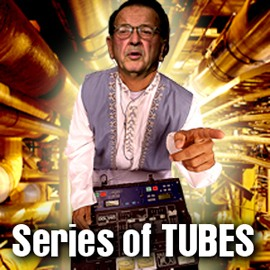
\includegraphics[width=3.4in]{figures/series-of-tubes.jpg}
\caption{This figure has several sub-figures.  a) shows a model with path shape and exterior connection point(s) brushed.  b) highlights the points which can't be tubed as drawn (if they are not connected, too tight, etc.).  c) shows our physics-based, energy-minimizing rod/tube and any path-smoothing that we do, d) shows the printed object with the tube (with something in it, EL wire presumably)}
\label{fig:tool-process-interior}
\end{figure}

take into account bend radius of desired material - no need, we just do the minimum-bending path

\subsubsection{Routing}

Our basic first-pass routing algorithm uses the A* routing algorithm \cite{Hart-Astar}.  The path cost in our implementation is based only on shortest distance between the starting and ending points, without weighting for distance from the surface.

Physical Simulation : 

How does it actually work?

Bend Minimization

Collision detection

\subsubsection{Mesh Modification}

How we actually cut stuff and make tubes happen.

\subsection{Fabrication Techniques}

\subsubsection{Printing} - different strategies with Objet (all print-in-place) and Makerbot (may need to add things like balloons afterwards).  Ryan just got flexible material, we should see how stretchy it is...!  We could also consider assembleable things that are easier to create using parts that clip together... probably out of scope.

\subsubsection{Hand Tools} - post-fabrication modification is possible using hand tools.  We can mark the surface to show where conduits are and how deep.  I can also use this to test things before spending time printing them using a big ol' block o' plastic.